\chapter{IBM High Level Assembler Language overview}

In general, high-level assemblers provide for their assembly languages features that are commonly found in high-level programming languages. Hence, in addition to ordinary machine instructions they also contain control statements similar to \textit{if, while, for} as well as custom callable macros.

IBM High Level Assembler (HLASM) comforts this definition and adds other features which will be described in this chapter.

\section{Syntax}

Because of historical reasons HLASM syntax is fairly complicated. Its line length is limited to 80 characters as it was in times when punch cards were used. 

Besides this HLASM uses syntax common to regular assemblers.

\subsection{Statement}

HLASM program is sequence of \textit{statements}. Statement consists of four fields. Those are:
\begin{itemize}
	\item \textbf{Name field} --- Serves as place for named constants that are to be used in code. The field is optional but when used it always starts in the first column of a line.
	
	\item \textbf{Operation field} --- Instruction that is executed. The only field that is mandatory. Must not begin in the first column as it would be interpreted as a name field.
	
	\item \textbf{Operands field} --- Field for instruction operands separated by comma located immediately after operation field. According to instruction used it can be any sequence of characters, apostrophe separated string or blank. 
	
	\item \textbf{Remark field} --- Serves as inline commentary. Optionally located after operands field or operation field when operands are blank.
\end{itemize}

This is an example of basic statement using all field.
\begin{verbatim}
 label   instruction     operands             remarks
.NOMOV       AGO     (&WH).L1,.L2,.L3     SEQUENTIAL BRANCH
\end{verbatim}

\subsection{Continuation}

One line in HLASM source code can contain only up to 80 characters. However, sometimes statement is too long to be written in one line. Therefore, special handling is introduced called \textbf{continuation}.

Firstly, let us elaborate more on the topic of line column. There are four special columns:
\begin{itemize}
	\item \textbf{Begin column (default 1)}
	
	\item \textbf{End column (default 71)}
	
	\item \textbf{Continuation column (default 72)}
	
	\item \textbf{Continue column (default 16)}
\end{itemize}
They all serve different purpose. First, \textit{begin column} states start of the statement or where name field should be written. Anything after \textit{end column} does not count as the content of a statement, rather it is used as a place for the line sequence number (see \ref{fig01:line}). 

\textit{Continuation column} is used for indication that statement continues on the next line (to indicate we write there arbitrary character other than space). Then the remainder of the statement must start on \textit{continue column} to finally create a well formed statement.

Here is an example of an instruction where its last operand exceeded 72.~column of the line.
\begin{verbatim}
  OP1                    REG12,REG07,REG04,REG00,REG01,REG11,Rx
        EG02
\end{verbatim} 
However, there are some instructions that allow so called \textit{extended format} of~operands allowing continuation even when line is not fully saturated.
\begin{verbatim}
  AIF   ('&VAR' FIND '~').A,     REMARK1                      x
        ('&VAR'  EQ  'L').B,     REMARK2                      x
        (T'&VAR  EQ  'U').C      REMARK3 
\end{verbatim} 
\begin{figure}[h]\centering
	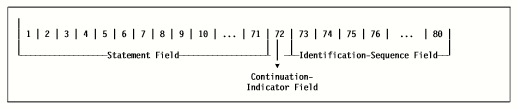
\includegraphics[scale=0.4]{img/line}
	\caption{Description of line columns (source HLASM Language Reference https://www-01.ibm.com/servers/resourcelink/\-svc00100.nsf/\-pages/\-zOSV2R3sc264940/\-\$file/\-asmr1023.pdf).}
	\label{fig01:line}
\end{figure}


\section{Assembling}

Having briefly described syntax, this section prepares reader to better understand assembly process hidden behind HLASM. 

We can divide this process into two interlinked steps, conditional assembly and ordinary assembly.

\subsection{Conditional assembly}

This part of assembly process can be compared to C++ text prepocessor. However, it is complicated process in HLASM and is commonly described as \textit{code generation}. It consists of \textbf{variable symbols}, \textbf{conditional assembly (CA) instructions} and \textbf{macros}. 


\subsubsection{Variable symbols}

These variables serves as points of substitution or information holders. 

When they occur in a statement, they are substituted by their value to create a new statement. For example, in this manner user can write variable symbol in operation field of statement and generate any instruction that can be a result of substitution.

Variable symbols have also notion of types. Symbol can be integer, boolean or string. CA instructions gather this information for different sorts of conditional branching.

\subsubsection{CA instructions}

The major difference to other instructions is that they are not assembled into object code, they rather choose which instructions will be. They are big contributors to \textit{code generation}.

One subset of CA instructions operates on variable symbols. With them user can define variable symbols locally or globally, assign or update their value.

Other subset is capable of conditional and unconditional branching. This is important in HLASM as you can alter flow of instructions that will be assembled into executable program.

\subsubsection{Macros}
Macro is structure consisting of name, input parameters and sequence of statements called body. When they are called in HLASM program, each statement in the body is performed. Nested or recursive call of macros is allowed. Macro body can even contain such sequence of instructions that it can generate another macro definition ready for later use. With help of variable symbols, HLASM macros have power to create custom task specific macros.

\subsection{Ordinary assembly}
